\documentclass[onecolumn]{hipatia}
\usepackage{array}
\newcommand{\PreserveBackslash}[1]{\let\temp=\\#1\let\\=\temp}
\newcolumntype{C}[1]{>{\PreserveBackslash\centering}p{#1}}
\newcolumntype{R}[1]{>{\PreserveBackslash\raggedleft}p{#1}}
\newcolumntype{L}[1]{>{\PreserveBackslash\raggedright}p{#1}}
\begin{document}
\pagestyle{empty}
\hspace{0pt}
\vfill
\begin{center}
	(Página intencionalmente deixada em branco.)
\end{center}
\vfill
\hspace{0pt}

\newpage

\pagestyle{empty}

\AddToHookNext{shipout/background}
 {%
  \put(2.2cm,-\paperheight+3cm)
{\begin{tikzpicture}
\meanderbox{8}{14}{0.72}
\end{tikzpicture}}
}
~\vspace{0.3cm}
\color{cinza}
\begin{center}
    {\fontsize{32}{32}\selectfont
    \scshape Cólofon}

\vspace{0.5cm}
Esta edição contou com a colaboração dos seguintes
alunos:

\begin{minipage}{12cm}
\vspace{0.2cm}
\begin{wrapfigure}{L}{1.5cm}
	\vspace{-10pt}
	\centering
	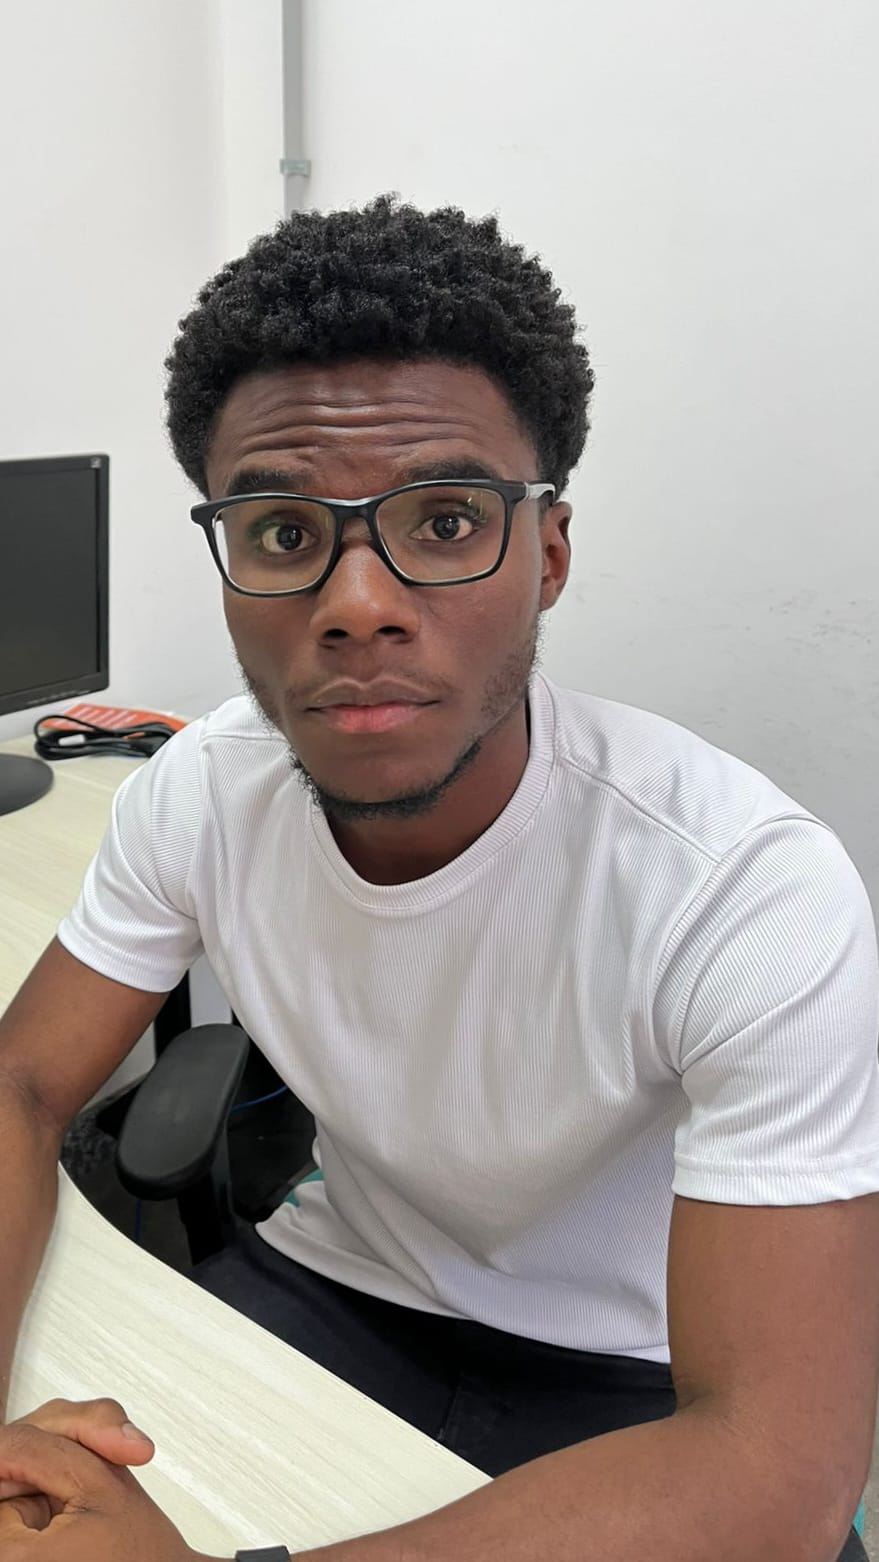
\includegraphics[width=2cm]{alisson.jpeg}
\end{wrapfigure}
Álisson Conceição Santos é egresso do IFBA, campus Salvador. Atualmente, é estudante de graduação em Matemática na UFBA, onde também é bolsista do PIBID. Além disso, Álisson atua como voluntário nas exposições do LEMA e integra o projeto de extensão Ondjango Asili. 
\end{minipage}
\begin{minipage}{12cm}
	\vspace{0.3cm}
\begin{wrapfigure}{L}{1.5cm}
	\vspace{-10pt}
	\centering
	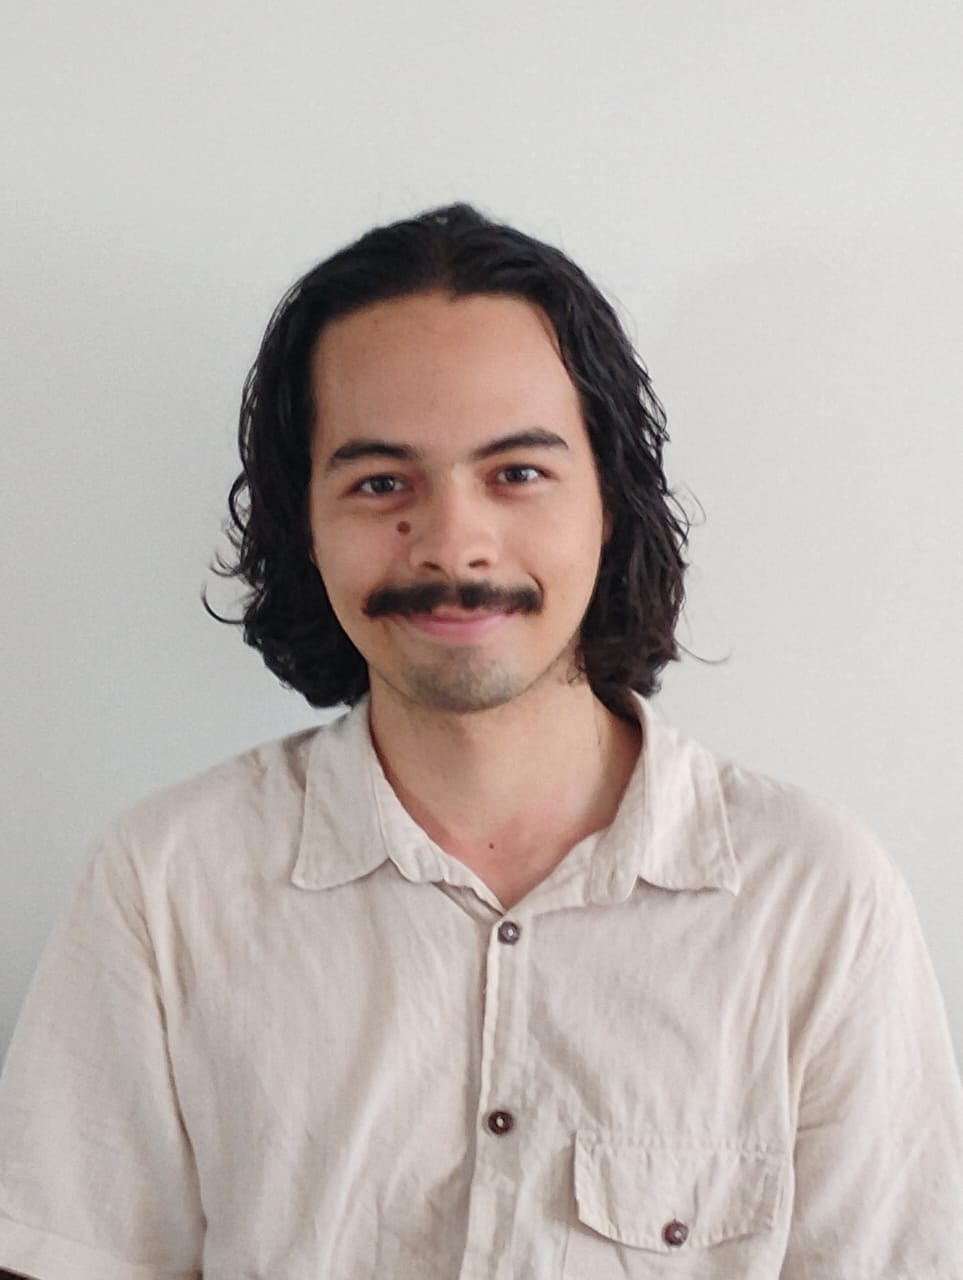
\includegraphics[width=2cm]{cleber.jpeg}
\end{wrapfigure}
Cleber Brito Figueiredo é estudante do bacharelado em física na Universidade Federal da Bahia (UFBA). Atualmente faz iniciação científica como bolsista da FAPESB em um projeto focado na teoria de Duffin-Kemmer-Petiau (DKP). Além disso, Cleber é apaixonado por jogos de tabuleiro e histórias de mistério.
\end{minipage}
\begin{minipage}{12cm}
	\vspace{0.3cm}
\begin{wrapfigure}{L}{1.5cm}
	\vspace{-10pt}
	\centering
	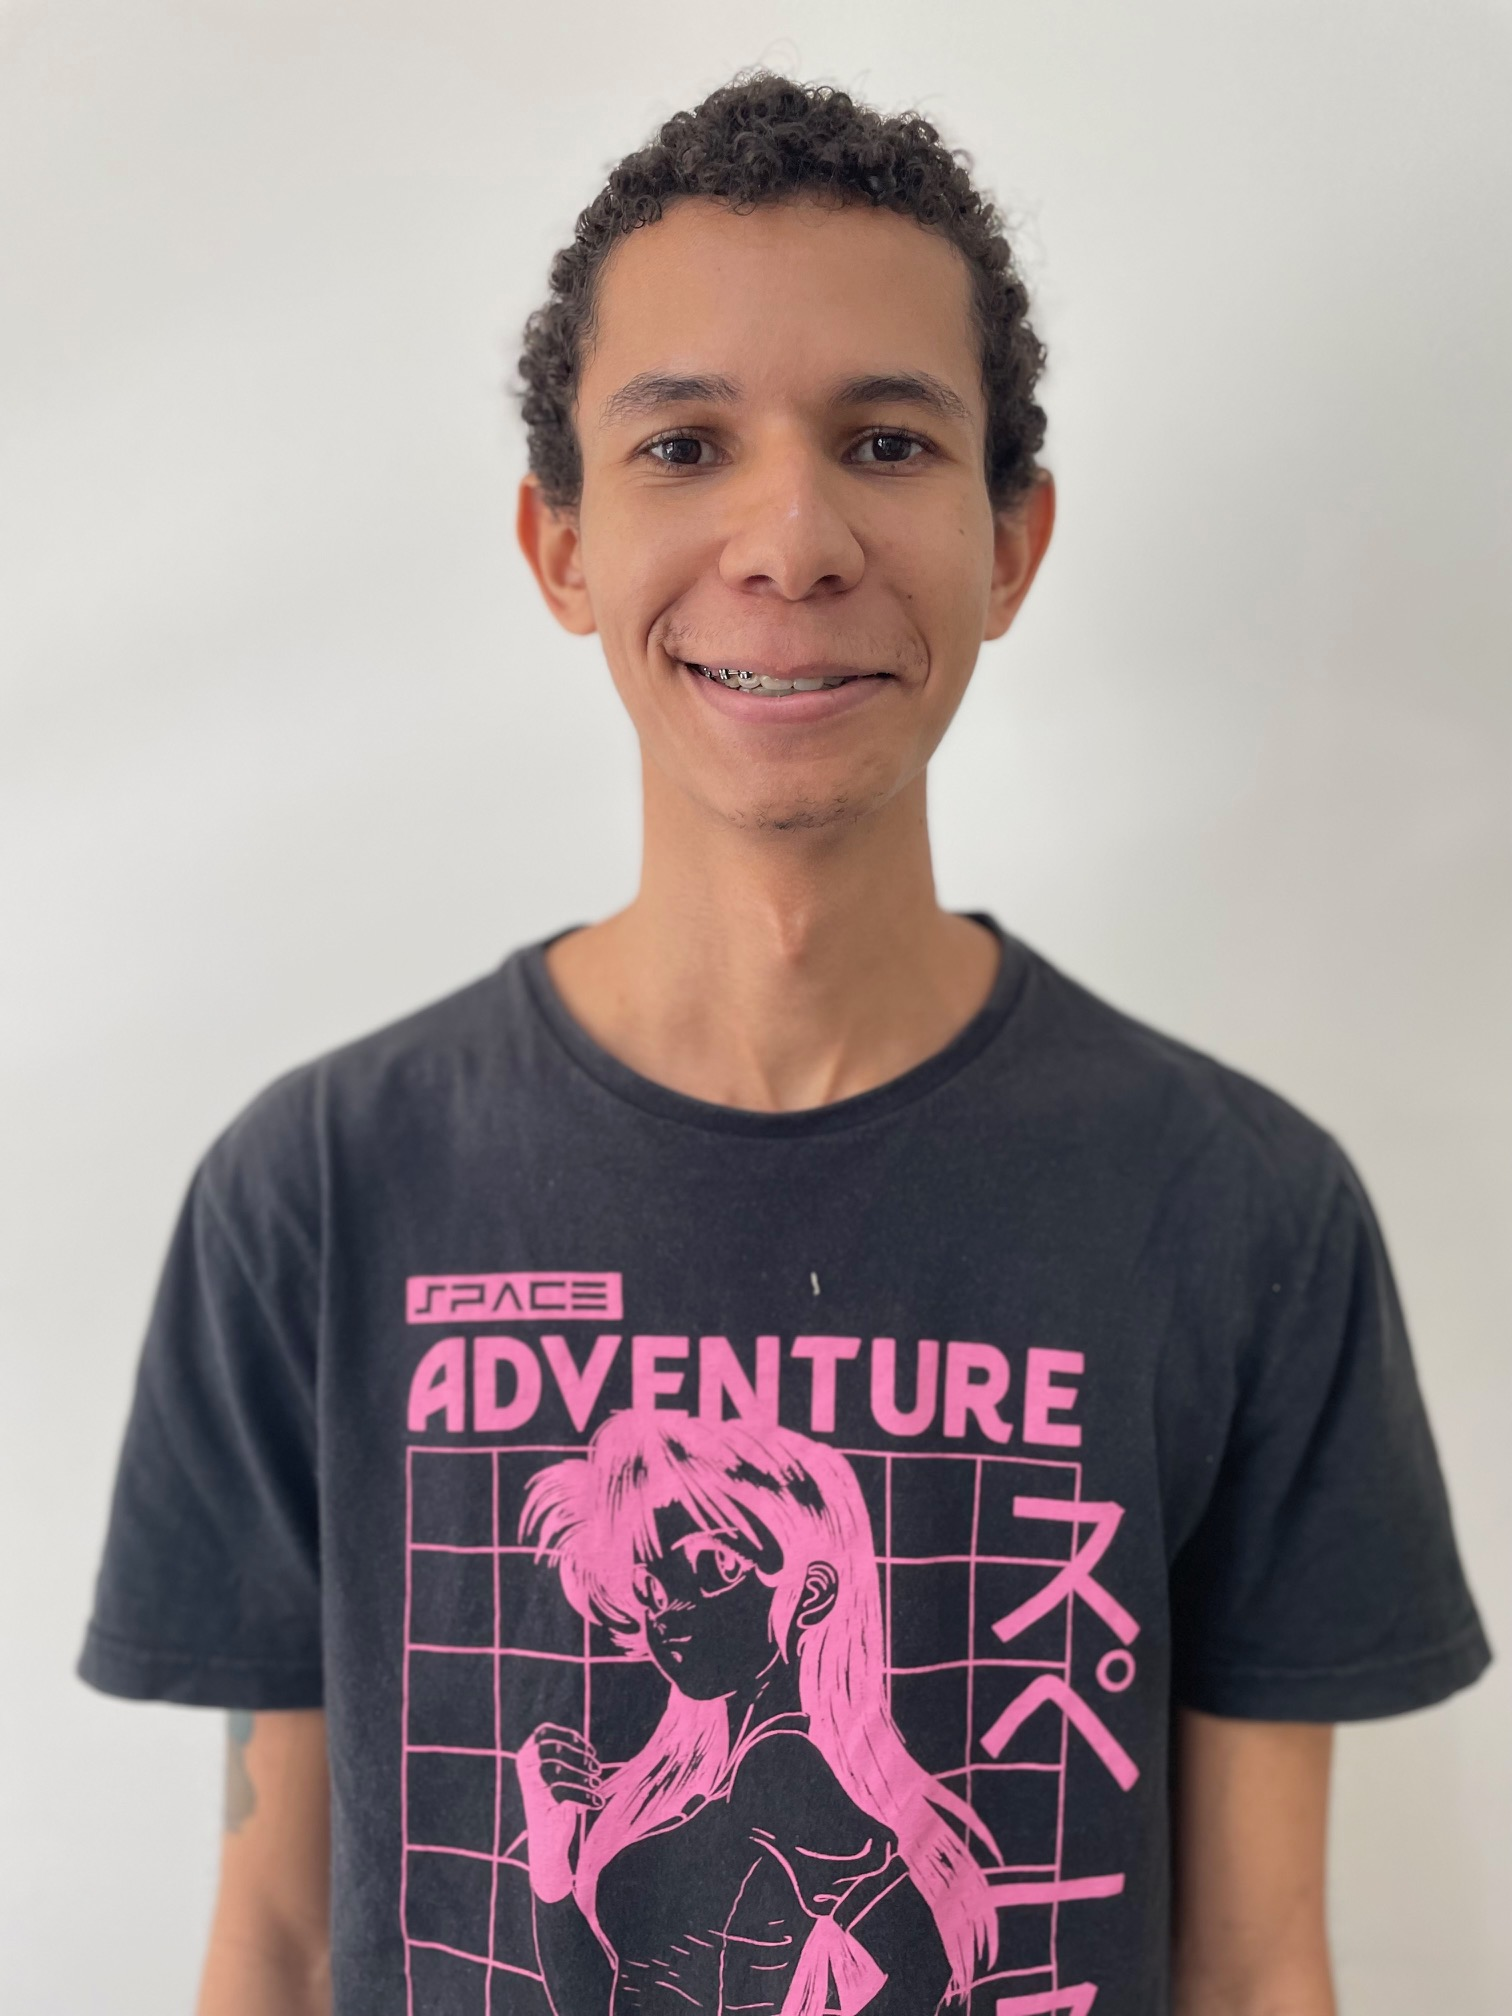
\includegraphics[width=2cm]{Eldon.png}
\end{wrapfigure}
Eldon Barros dos Reis Júnior é bacharel 
em Matemática pela Universidade Federal da Bahia (UFBA) 
e atua como bolsista no Programa Institucional de 
Bolsas de Iniciação Científica (PIBIC) na área de Probabilidade com o projeto
``Método da Entropia Relativa e $q$-Entropia''.
\end{minipage}
\begin{minipage}{12cm}
	\vspace{0.3cm}
	\begin{wrapfigure}{L}{1.5cm}
		\vspace{-10pt}
			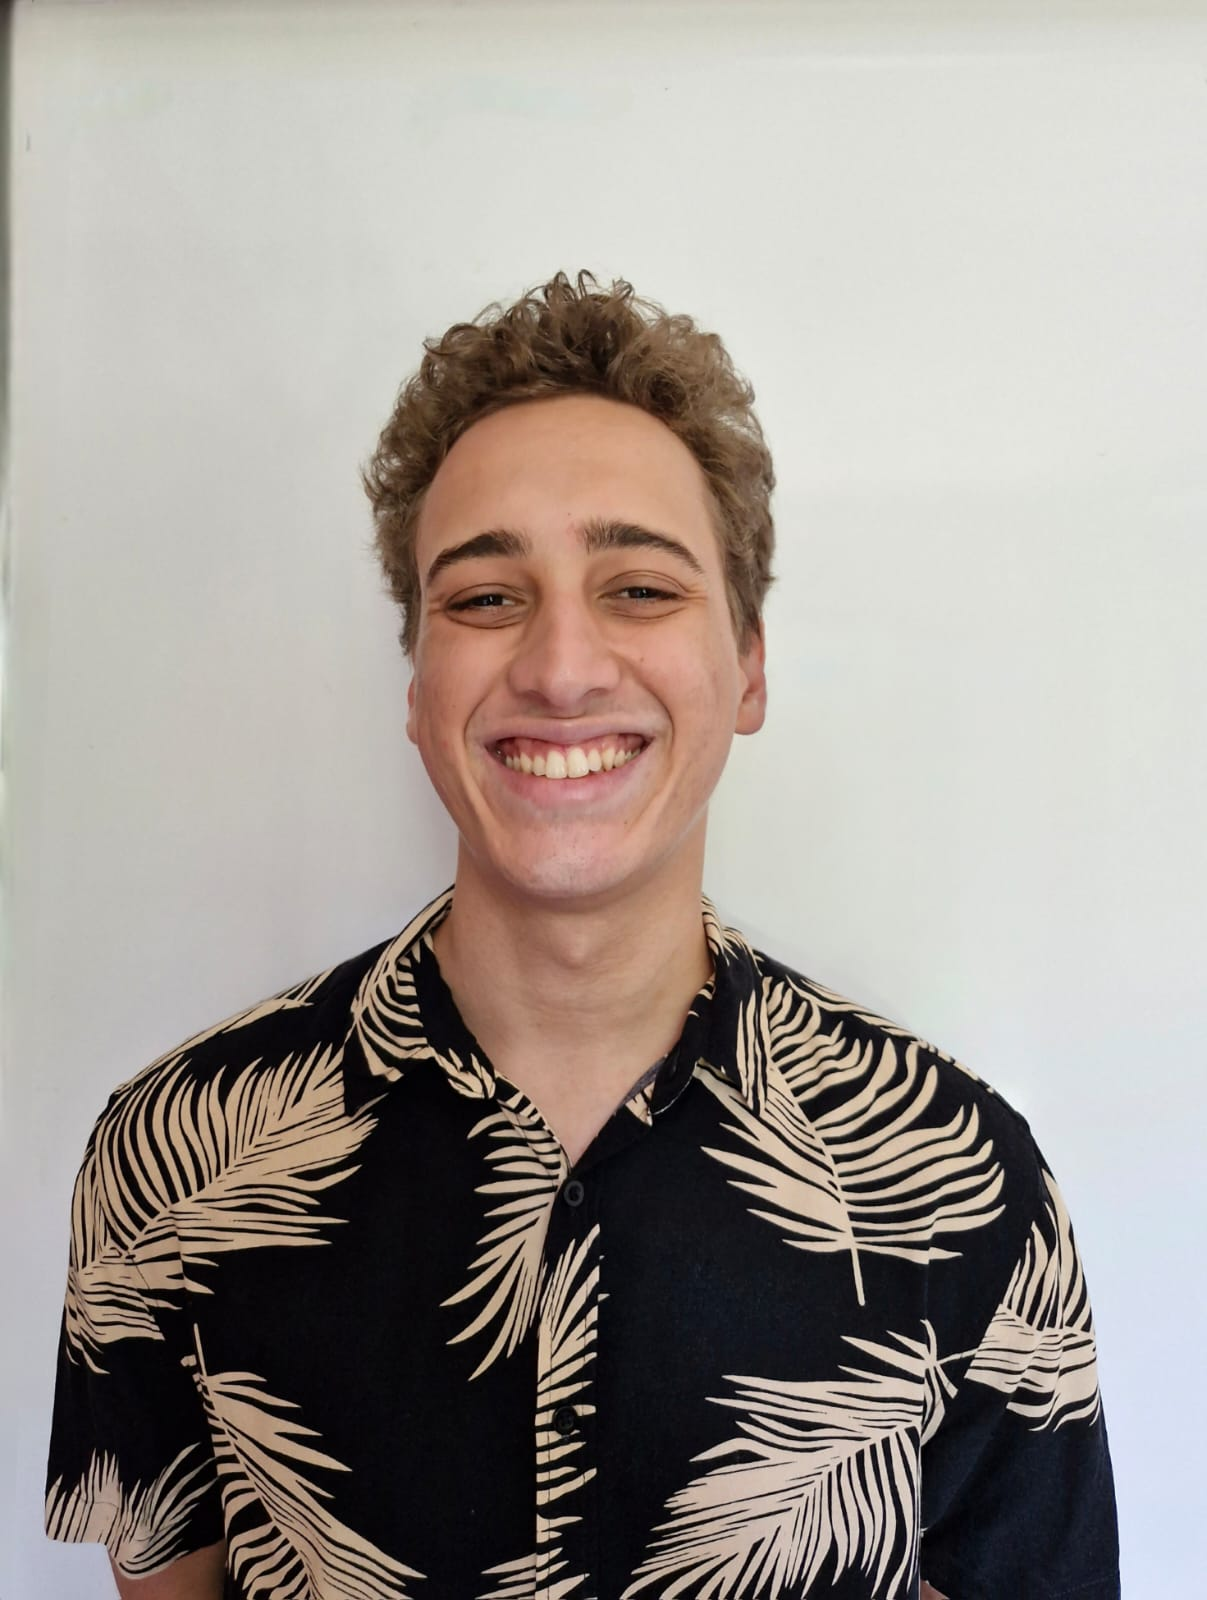
\includegraphics[width=2cm]{joao.jpeg}
		\end{wrapfigure}
		João Vitor Fonseca iniciou sua trajetória acadêmica no curso de engenharia elétrica, com uma longa passagem na medicina e, por fim, na matemática, onde hoje cursa bacharelado. Realizou pesquisas na área de epidemiologia e patologia digital, quando foi bolsista do programa PIBIC. Além da matemática, tem grande interesse em música, entusiasta da improvisação.
	\end{minipage}
	\begin{minipage}{12cm}
		\vspace{0.3cm}
		\begin{wrapfigure}{L}{1.5cm}
			\vspace{-10pt}
				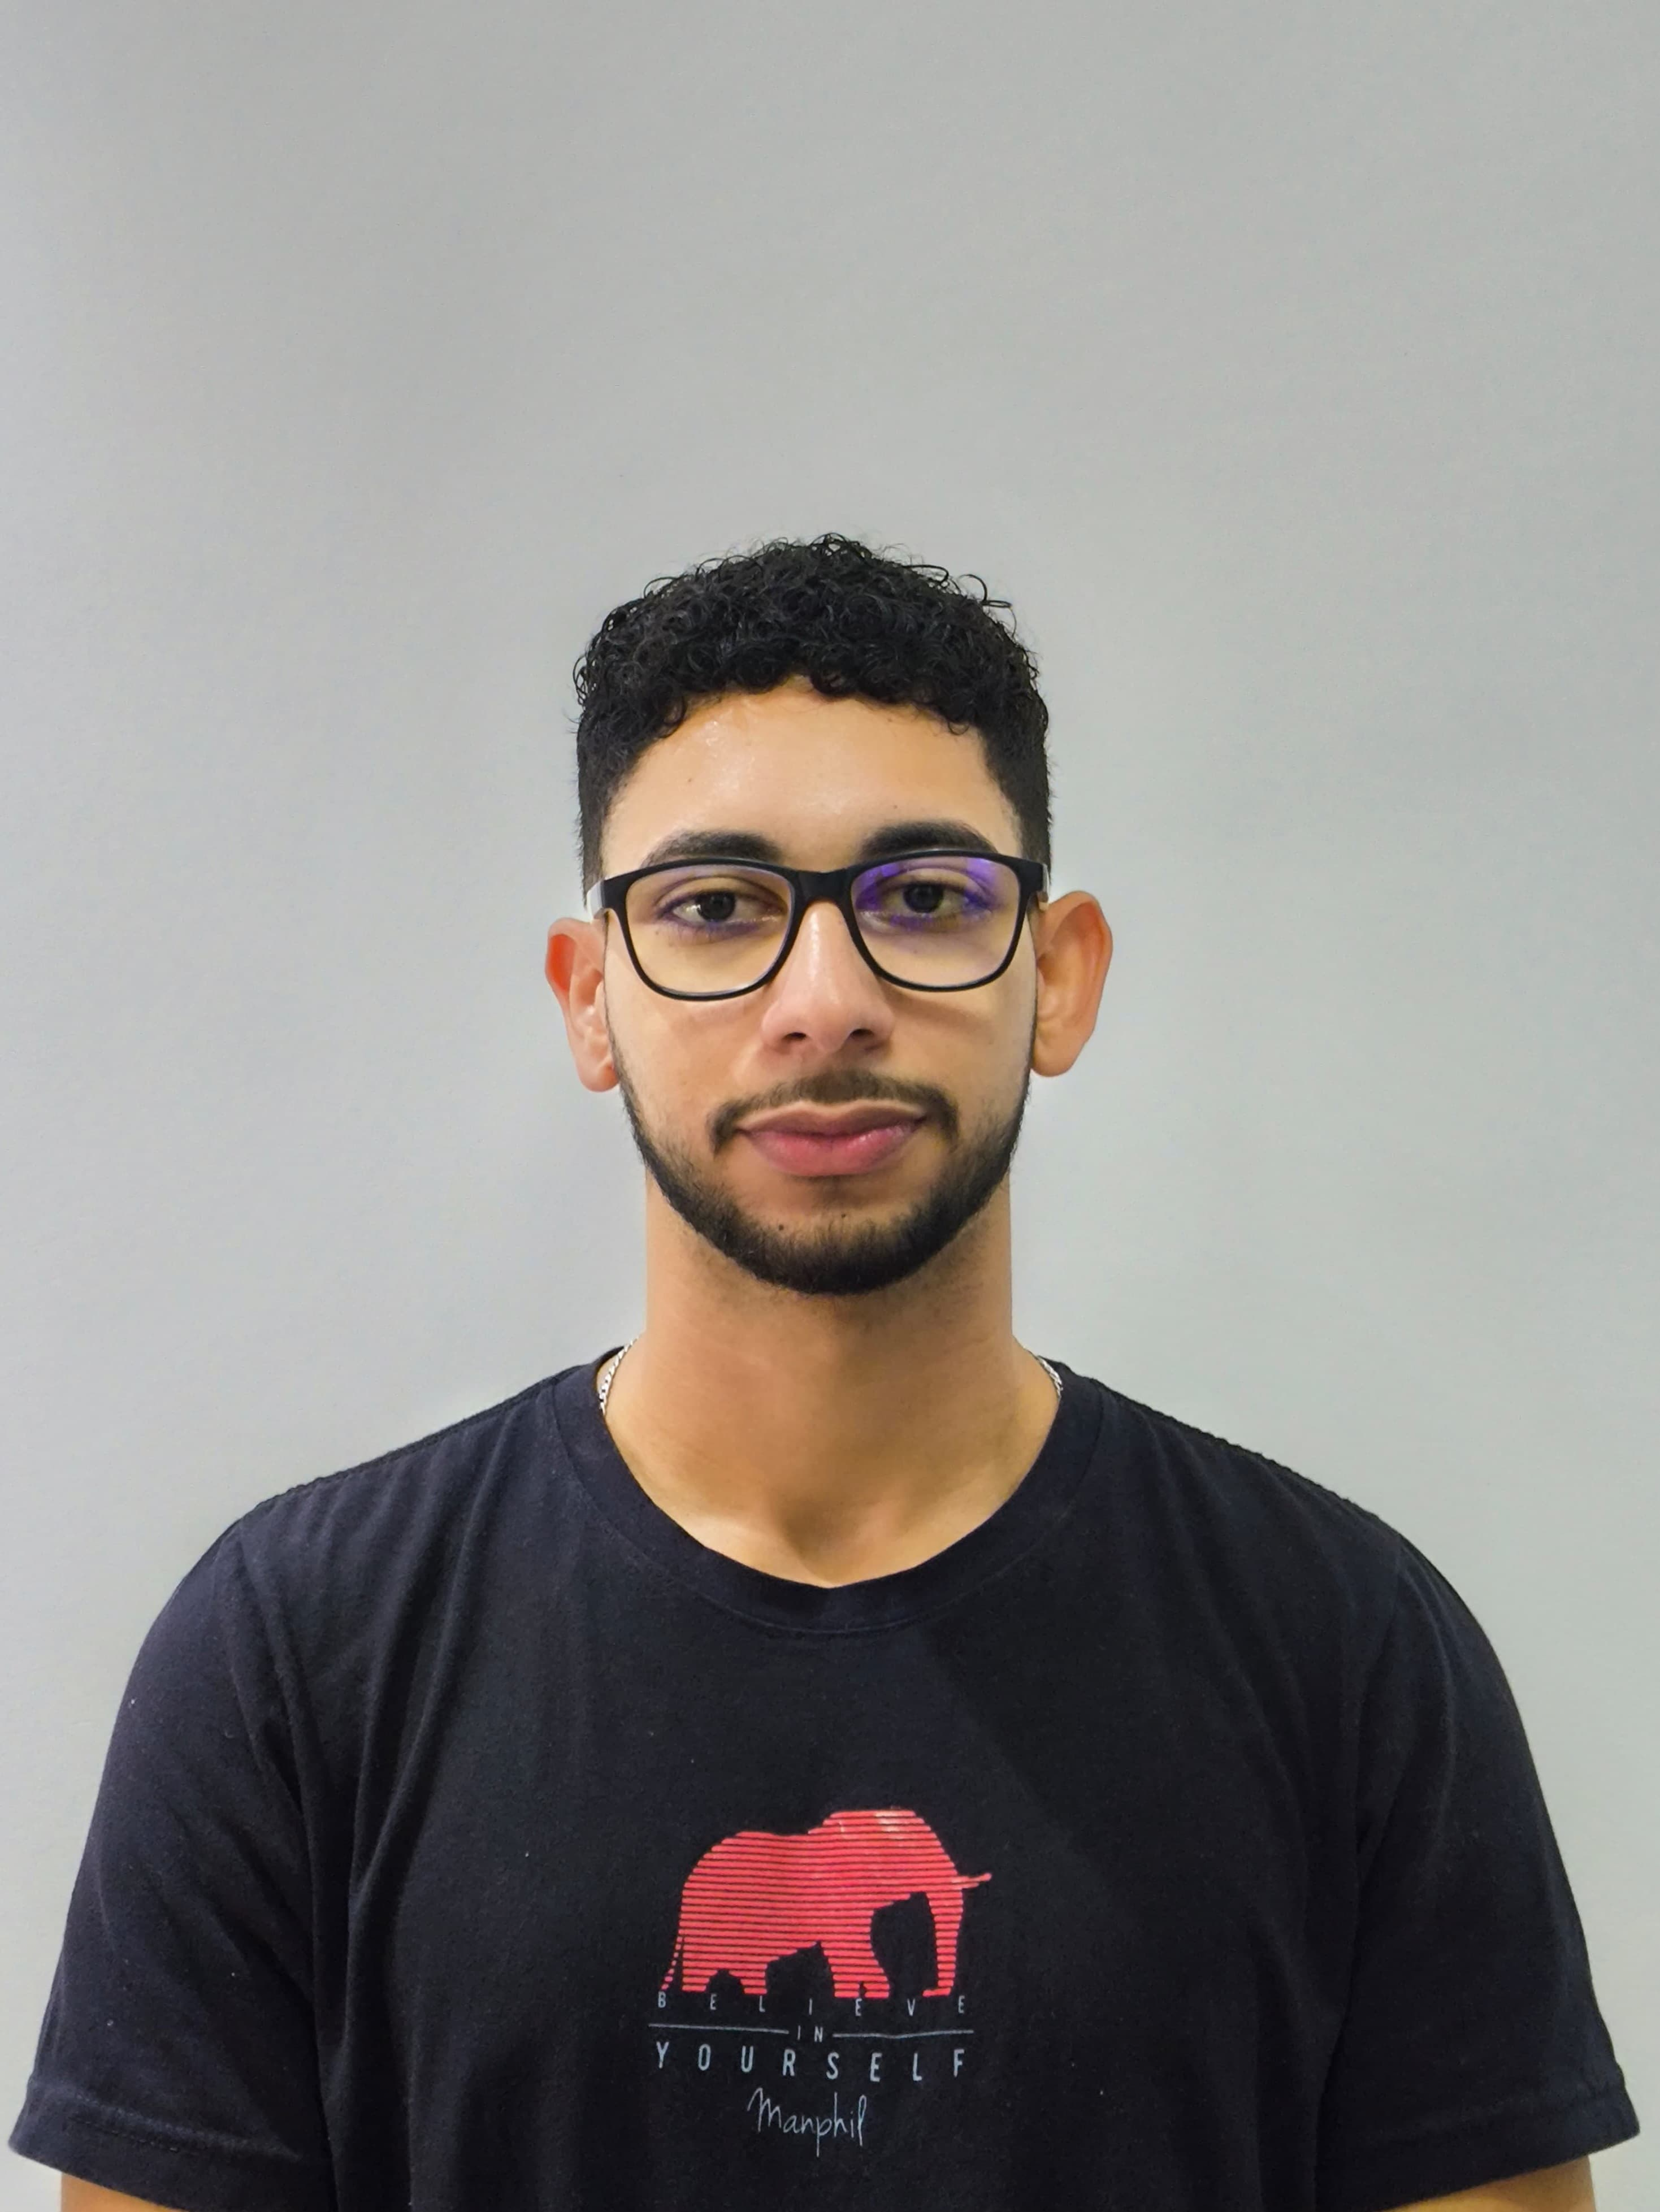
\includegraphics[width=2cm]{jose.jpeg}
			\end{wrapfigure}
			José Valdomiro da Silva Neto é estudante do bacharelado em estatística na UFBA. Assistente de esportes na Associação Acadêmica Atlética Alan Turing e monitor voluntário nas exposições do LEMA, José está apenas começando sua jornada na universidade.
		\end{minipage}	
\begin{minipage}{12cm}
	\vspace{0.3cm}
	\begin{wrapfigure}{L}{1.5cm}
		\vspace{-10pt}
		\centering
		
\includegraphics[width=2cm]{Taise.jpg}
	\end{wrapfigure}
	Taíse Lara de Souza Jorge é licenciada em Matemática pela UFBA 
	e mestranda em Educação pela UFFS. Realiza pesquisa na área de Mediação
	Pedagógica e Alfabetização Matemática sob a perspectiva do Numeramento, 
	amparada na Educação Crítica e Educação Matemática Crítica. 
\end{minipage}
\begin{minipage}{12cm}
	\vspace{0.3cm}
	\begin{wrapfigure}{L}{1.5cm}
		\vspace{-10pt}
		\centering
		
\includegraphics[width=2cm]{yure.jpeg}
	\end{wrapfigure}
	Yure Carneiro de Oliveira graduou-se e fez mestrado em matemática na UFBA, onde também realiza seu doutorado em matemática na área de Probabilidade. Após quase concluir um mestrado em estatística, ingressar em uma outra graduação e começar a estudar violino, agora está focado na conclusão do doutorado.
\end{minipage}

\end{center}



\newpage

\pagestyle{empty}
\pagecolor{olivalight}
~
\vfill
\begin{center}
	\includegraphics[width=9cm]{Logos_contracapa_Hipátia_2.jpeg}

	\vspace{4cm}

	
\includegraphics[width=4cm]{QR.png}
	
	Link para o \emph{site} da
	
	Revista de Matemática Hipátia

\end{center}

\vfill
\newpage
\AddToHookNext{shipout/background}
 {%
  \put(0,-\paperheight)
{\begin{tikzpicture}
\meanderbox{8}{13}{0.888}
\end{tikzpicture}}
}

~\\[4cm]
\begin{center}
	
\includegraphics[width=10cm]{Hipatiaazul.png}
\end{center}


\end{document}